\documentclass[5pt]{article}
\usepackage{mathptmx,amsmath}
\usepackage{pdfslide2,pause}
\usepackage{eurosym}
\usepackage[portuguese,english]{babel}
\usepackage{kerkis}
\usepackage{colortbl} % used to highlight row or columns of tables. http://www.tug.org/pracjourn/2007-1/mori/mori.pdf
\usepackage[small]{caption} % more option on http://www.dd.chalmers.se/latex/Docs/PDF/caption.pdf
\usepackage[tight,scriptsize]{subfigure}
\usepackage{lastpage}
\usepackage{chngcntr}
\usepackage[absolute,overlay]{textpos}
\usepackage{tabto}
\usepackage{animate}
%\usepackage{listings}
\captionsetup{labelformat=empty,skip=-0.8cm}

%\lstset{
%    language=Matlab,                % choose the language of the code
%    basicstyle=\ttfamily\tiny,       % the size of the fonts that are used for the code
%    numbers=none,                   % where to put the line-numbers
%    numberstyle=\tiny,              % the size of the fonts that are used for the line-numbers
%    stepnumber=1,                   % the step between two line-numbers. If it's 1 each line will be numbered
%    numbersep=5pt,                  % how far the line-numbers are from the code
%    backgroundcolor=\color{white},  % choose the background color. You must add \usepackage{color}
%    showspaces=false,               % show spaces adding particular underscores
%    showstringspaces=false,         % underline spaces within strings
%    showtabs=false,                 % show tabs within strings adding particular underscores
%    tab=\rightarrowfill,
%    frame=none,	                    % adds a frame around the code
%    tabsize=2,	                    % sets default tabsize to 2 spaces
%    captionpos=b,                   % sets the caption-position to bottom
%    breaklines=true,                % sets automatic line breaking
%    breakatwhitespace=false,        % sets if automatic breaks should only happen at whitespace
%    title=\lstname,                 % show the filename of files included with \lstinputlisting; also try caption instead of title
%    escapeinside={\%*}{*)},          % if you want to add a comment within your code
%    morekeywords={ifftshift,fftshift},
%    keywordstyle=\bfseries\color[rgb]{0,0,0.3},
%    commentstyle=\color[rgb]{0.133,0.5,0.133}
%}
%\lstset{
%    emph={function,end,for,if,while},
%    emphstyle=\bfseries\color[rgb]{0.6,0,0},
%}

\definecolor{itblue}{rgb}{0.0,0.0,0.5}
\definecolor{itred}{rgb}{0.82,0.18,0.24}
\newcommand{\pageNum}{
    \begin{picture}(0,0)(0,0)
        \put(-15,-390){
            \begin{minipage}{1.8cm}
            \end{minipage}
        }
    \end{picture}
}
\newcommand{\cb}[1]{{\color{itblue} #1}}%
\newcommand{\cred}[1]{{\color{itred} #1}}%
\newcommand{\bb}[1]{{\textbf{\color{itblue} #1}}}%
\newcommand{\br}[1]{{\textbf{\color{itred} #1}}}%
\renewcommand{\labelitemi}{\textcolor{itred}{\normalsize $\bullet$}}
\renewcommand{\labelitemii}{\textcolor{itblue}{$\bullet$}}
\newcommand{\mysection}[1]{\section*{\pageNum\color{itred}\sffamily #1}\vspace*{0.5cm}\overlay{it_1.png}\sffamily}%
\newcommand{\ITfootnote}[1]{\hspace{1.8cm}\begin{minipage}{13cm}\tiny{#1}\end{minipage}}
\newcommand{\edfaGain}{$G=\exp\left(\frac{\alpha}{2}L_{span}\right)$}
\newenvironment{reference}{
    \begin{textblock*}{0.7\textwidth}(32mm,137mm)\tiny\noindent\bgroup\color{black}
}
{
    \egroup\end{textblock*}
}


\graphicspath{{./Figures/}}
\pagestyle{title}

\hyphenpenalty=50000
\tolerance=10000

\setlength{\textheight}{1.5\textheight}

%%%%%%%%%%%%%%%%%%%%%%%%%%%%%%%%%%%%%%%%%%%%%%%%%%%%%%%%%%%%%%%%%%%%%%%%%%%%%%%%%%%%%%%%%%%%%%%%%%%
%%%%%%%%%%%%%%%%%%%%%%%%%%%%%%%%%%%%%%%%%%%%%%%%%%%%%%%%%%%%%%%%%%%%%%%%%%%%%%%%%%%%%%%%%%%%%%%%%%%

\begin{document}

%************************************************************************************************
%                                          SLIDE
%************************************************************************************************
\pagenumbering{roman}
\begin{titlepage}  \overlay{it_0.png}

\color{itblue} \sffamily \noindent \small
\hspace*{1cm}  Universidade de Aveiro\\ %Instituto\\ Superior T�cnico, Instituto de Telecomunica��es\\
\hspace*{1cm}  2017-2018\\ %Lisboa, 14th of February, 2013\\

\vspace*{1cm}
\begin{center}
    \color{black} \sffamily \noindent \Large
    \br{Quantum Oblivious Key Distribution with Discrete Variables\\}
\end{center}
\vspace{6mm}
\begin{center}
    \color{black}
    \textbf{Mariana Ferreira Ramos\\}
    {(marianaferreiraramos@ua.pt)}
\end{center}

\vspace{0.0mm}
\scriptsize
\begin{center}
Department of Electronics, Telecommunications and Informatics,\\
University of Aveiro, Aveiro, Portugal\\
Instituto de Telecomunica\c{c}\~{o}es, Aveiro, Portugal\\
\end{center}

\vspace{1.0cm}
\hspace*{13.2cm}\tiny \copyright 2005, it - instituto de telecomunica\c{c}\~{o}es\hfill

\end{titlepage}


\renewcommand{\headsep}{-25pt}
\pagenumbering{arabic}



%--------------------------------------------------------------------------------------------------
%------------ SLIDE-------
\mysection{Quantum Oblivious Key Distribution System (QOKD)}\large
\vspace{0cm}

    The QOKD system enables two parties (Alice and Bob) to share a set of keys. These keys have the particularity of being half right and half wrong. Only Bob knows which are right and wrong bits. Alice only knows that at some tabs there are the same number of right and wrong measurements.

    \begin{figure}[hbt]
    	\centering
    	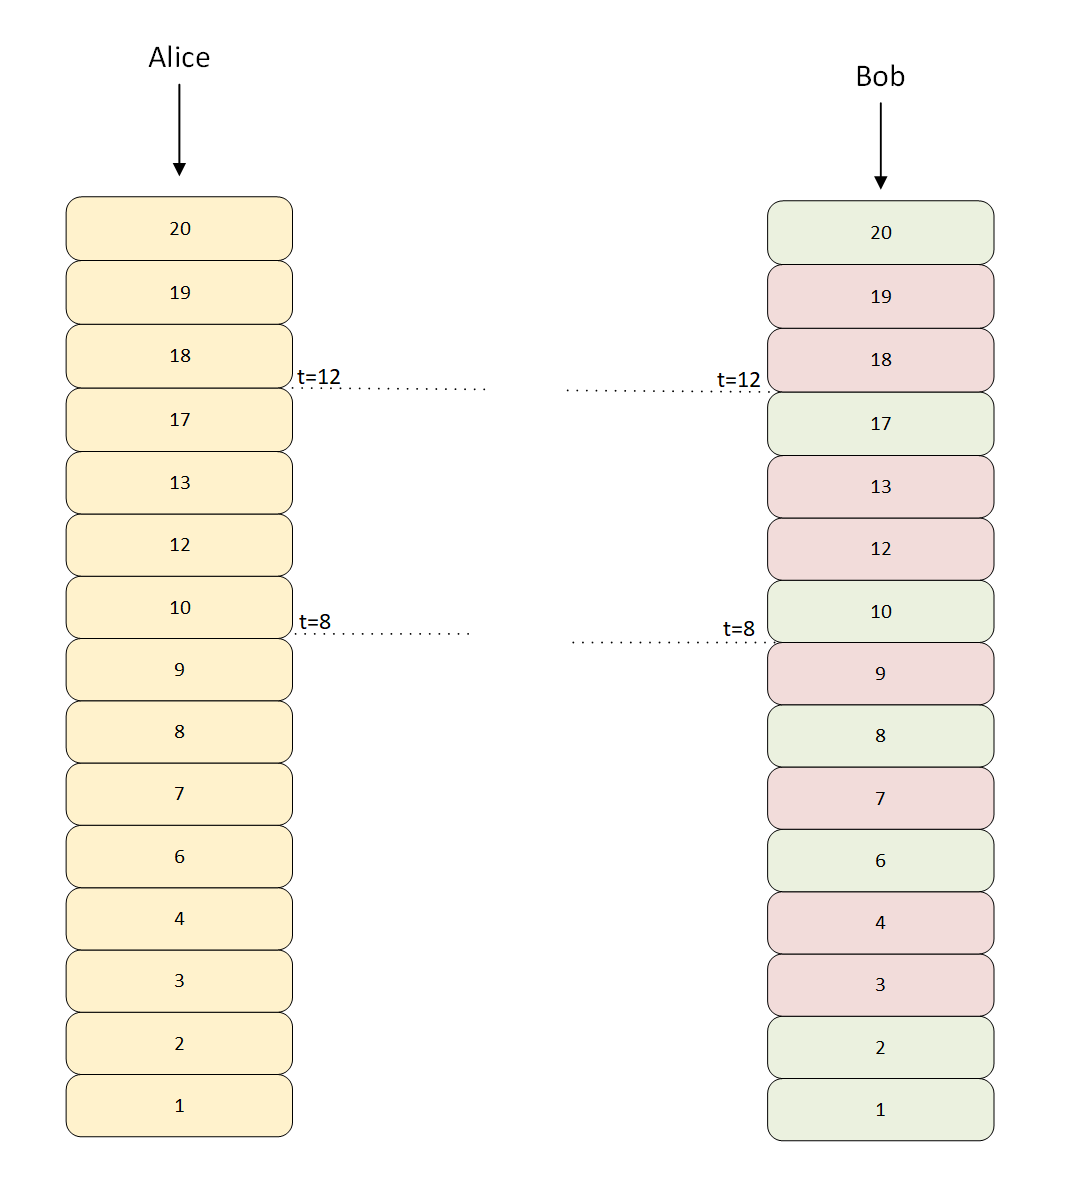
\includegraphics[width=0.6\textwidth, height=7cm]{./figures/alicebobkeys.png}
        	\label{alicebobkeys}
    \end{figure}

%--------------------------------------------------------------------------------------------------
%------------ SLIDE -------------------------------------------------------------------------------

\mysection{ \\[-5mm]1-out-of-2 OT Protocol: starting conditions}\large
\vspace*{0mm}
\begin{itemize}
    \item {Alice has two messages $m_1$ and $m_2$ and Bob wants to know one of them, $m_b$, without Alice knowing which one, i.e. without Alice knowing $b$, and Alice wants to keep the other message private, i.e. without Bob knowing $m_{\bar{b}}$.}\\[-5mm]
    \item {In order to implement OT between two parties (Alice and Bob) they must be able to exchange continuously oblivious keys, i.e a QOKD system must exist between them.}
    \item {Two basis are required: $'+'$ rectilinear basis and $'\times'$ diagonal basis. Lets assume,}

    \begin{center}
    \begin{tabular}{c|c}
            & Basis "+" \\ \hline
         0 & $\to (0^{\circ})$ \\
         1 & $\uparrow (90^{\circ})$ \\
    \end{tabular}
    \quad
    \begin{tabular}{c|c}
          & Basis "$\times$" \\ \hline
         0 & $\searrow (-45^{\circ})$ \\
         1 & $\nearrow (45^{\circ})$ \\
    \end{tabular}

\end{center}
\end{itemize}


%--------------------------------------------------------------------------------------------------
%------------ SLIDE--------------------------------------------------------------------------------
\mysection{1-out-of-2 OT Protocol with QOKD system}\large
\vspace{0cm}
Lets assume Alice sends the following two messages with size $s=4$, $m_{0} = \{0 0 1 1\}$ and $m_{1} = \{0 0 0 1\}$. At $t=8$ Alice does not need to eliminate any bits.
\begin{description}
  \item[Step 1] Bob defines two sub-sets with size $s=4$:
  $$I_{0}=\{3,4,7,9 \},$$
  and $$I_{1}= \{1,2,6,8 \},$$ where $I_{0}$ is the sequence of positions in which Bob was wrong about basis measurement and $I_{1}$ is the sequence of positions in which Bob was right about basis measurement.


\end{description}

%--------------------------------------------------------------------------------------------------
%------------ SLIDE--------------------------------------------------------------------------------
\mysection{1-out-of-2 OT Protocol with QOKD system}\large
\vspace{0.4cm}
\begin{description}
  \item[Step 2] Bob sends to Alice the set $S_{b}$. Lets assume he wants to know $m_{0}$, therefore he sends $S_{0}=\{I_{1},I_{0} \}$. Alice is sure about Bob's honesty, since she knows he only has $4$ right basis to measure the photons. In addition, Alice cannot know which message Bob chose because she did not know the order that he sent the sets.
  \item[Step 3] Alice defines two encryption keys $K_{0}$ and $K_{1}$ using the values in positions defined by Bob in the set sent by him. Lets assume, $$K_{0}=\{1,1,1,0\}$$ $$K_{1}=\{0,0,0,1\}.$$ Alice does the following operations:
   $$m = \{m_{0}\oplus K_{0}, m_{1} \oplus K_{1} \}.$$

\end{description}



%--------------------------------------------------------------------------------------------------
%------------ SLIDE--------------------------------------------------------------------------------
\mysection{1-out-of-2 OT Protocol with QOKD system}\large
\vspace{0.4cm}
\begin{description}
  \item[Step 3 -cont ] Alice sends to Bob through a classical channel $$m=\{1,1,0,1,0,0,0,0\}.$$

  \item[Step 4] Bob uses $S_{B1\prime}$ values of positions given by $I_{1}$ and $I_{0}$ and does the decrypted operation.

   \begin{table}[hbt]
        \centering
        \begin{tabular}{c|c c c c c c c c}
         $m$ & 1 & 1 & 0 & 1 & 0 & 0 & 0 & 0 \\
             & 1 & 1 & 1 & 0 & 0 & 1 & 1 & 0 \\ \hline
         $\oplus$ & 0 & 0 & 1 & 1 & 0 & 1 & 1 & 0 \\
        \end{tabular}
        \end{table}
    The first four bits corresponds to message 1 and he received $\{0,0,1,1\}$, which is the right message $m_{0}$ and $\{0,1,1,0\}$ which is a wrong message for $m_{1}$.
\end{description}

%--------------------------------------------------------------------------------------------------
%------------ SLIDE-------
\mysection{Quantum Oblivious Key Distribution System (QOKD)}\large
\vspace{0cm}

\begin{itemize}

  \item Alice randomly generates the following sets $S_{A1'}$ (for basis) and $S_{A2'}$ (for keys) in order to encode photons.
  \item  Alice sends to Bob throughout a quantum channel $l$ photons encoded using the previous values,

   $$S_{AB} = \{\uparrow ,\uparrow ,\nearrow ,\searrow,\searrow, \to , \to, \searrow,\nearrow,\uparrow , \to ,\searrow,\nearrow,\searrow ,\uparrow ,\nearrow \}$$

   \item Bob also randomly generates $l=16$ bits, which are going to define his measurement basis, $S_{B1'}$,
   $$  S_{B1'}= \{ +,\times,\times,+,+,\times,+,\times, \times,+, \times, \times \,+,+,+,\times \}.$$
\end{itemize}

%--------------------------------------------------------------------------------------------------
%------------ SLIDE-------
\mysection{Quantum Oblivious Key Distribution System (QOKD)}\large
\vspace{0cm}
\begin{itemize}

  \item After measure the photons using the basis generated in $S_{B1'}$ , he got $S_{B2'}$:
  
      \begin{table}[hbt]
        \centering
        \begin{tabular}{c|cccccccccccccccc}
        \hline \\
        \textbf{$S_{AB}$}  & $\uparrow$ & $\uparrow$ & $\nearrow$      & $\searrow$ & $\searrow$ & $\to$    & $\to$           & $\searrow$ & $\nearrow$ & $\uparrow$ & $\to$    & $\searrow$ & $\nearrow$ & $\searrow$ & $\uparrow$      & $\nearrow$ \\
        \textbf{$S_{B1'}$} & $+$        & $\times$   & $\times$        & $+$        & $+$      & $\times$ & $+$             & $\times$   & $\times$   & $+$        & $\times$ & $\times$   & $+$        & $+$        & $+$             & $\times$   \\
        \textbf{$S_{B2'}$} & $1$        & $-$        & $\underline{0}$ & $0$          & $-$      & $1$      & $\underline{1}$ & $-$        & $1$        & $-$        & $1$      & $0$        & $1$        & $1$        & $\underline{0}$ & $1$ \\ \\\hline
        \end{tabular}
      \end{table}
      where "$-$"\space{ } corresponds to no clicks in Bob's detector, due to attenuation and the underlined values to measurements with a correct basis but an error has occurred due to imperfections in the quantum communication system.

\end{itemize}

%--------------------------------------------------------------------------------------------------
%------------ SLIDE-------
\mysection{Quantum Oblivious Key Distribution System (QOKD)}\large
\vspace{0cm}
\begin{itemize}
\item Bob sends to Alice, $$S_{BH1}=\{{S}_{1},-1,{S}_{2},{S}_{3}, -1,{S}_{4},{S}_{5},-1,{S}_{6},-1,{S}_{7},{S}_{8},{S}_{9},{S}_{10},{S}_{11},{S}_{12} \},$$ where "$-1$" correspond to no clicks at the detector and the other values are Hash values calculated using SHA256.
  \item After Alice has received $S_{BH1}$, she sends throughout a classical channel the basis which she has used to codify the photons updated with the information about the no received photons.
   \item  This way, due to attenuation them sets are reduced,
    $$S_{A1}=\{0,1,1,0,0,1,0,1,1,1,0,1 \}, \ S_{A2}=\{1,1,0,0,0,1,0,0,1,0,1,1 \},$$
      $$S_{B1}=\{0,1,0,1,0,1,1,1,0,0,0,1 \}, \ S_{B2}=\{1,\underline{0},0,1,\underline{1},1,1,0,1,1,\underline{0},1 \}$$
 


\end{itemize}

%--------------------------------------------------------------------------------------------------
%------------ SLIDE-------
\mysection{Quantum Oblivious Key Distribution System (QOKD)}\large
\vspace{0cm}

\begin{itemize}
    
 \item Then, they apply a modified version of Cascade Algorithm in order to correct errors due transmission in the right set of measurements. Furthermore, they test the honesty of each other using the estimated QBER from Alice and the Hash Function committed by Bob.
      
  \item In order to know which photons were measured correctly, Bob does the operation $S_{B3}=S_{B1} \oplus S_{A1}$.
  \item Bob got $S_{B3} = \{1,1,0,0,1,1,0,1,0,0,1,1 \}.$
  \item The values "1" correspond to the values he measured correctly and "0" to the values he just guessed.
  \item Bob is building two sets of keys, one with correct basis measurements values and other with the wrong basis measurement values that he just guessed.
  
\end{itemize}
%--------------------------------------------------------------------------------------------------
%------------ SLIDE-------
\mysection{Quantum Oblivious Key Distribution System (QOKD)}\large
\vspace{0cm}
\begin{itemize}

  \item  By the end, Bob has four sets in order to have the capability of decode messages sent by Alice:
    \begin{align*}
        S_{B_{rp}} & = \{1,2,5,6,8 \} \\
        S_{B_{rb}} & = \{1,1,0,1,0 \} \\
        S_{B_{wp}} & = \{3,4,7,9 \} \\
        S_{B_{wb}} & = \{0,1,1,0 \}
      \end{align*}
\end{itemize}

%-------------------------------------------------------------------
%------------ SLIDE ------------------------------------------------
\mysection{} \sffamily
\vspace{-10mm}
\large\centerline{E-mail: marianaferreiraramos@ua.pt}


\end{document}
